\documentclass[11pt,a4paper]{article}
\usepackage[margin=0.9in]{geometry}
\usepackage[T1]{fontenc}
\usepackage[utf8]{inputenc}
\usepackage{mathptmx,amsmath,amssymb,graphicx,booktabs,tabularx,placeins,indentfirst,authblk}
\renewcommand\Authfont{\normalsize}
\renewcommand\Affilfont{\small\itshape}
\setlength{\affilsep}{0.6em}
\newcolumntype{Y}{>{\raggedright\arraybackslash}X}
\usepackage[font=small,labelfont=bf]{caption}
\usepackage[hidelinks,breaklinks=true]{hyperref}
\hypersetup{pdftitle={Real Data Anchoring and Sampling Bias in Recursive Training of Imbalanced Gaussian Mixtures},pdfauthor={GAO Jiashen, TONG Yizhou}}
\setlength{\parindent}{1.15em}
\setlength{\parskip}{2pt}
\setlength{\textfloatsep}{12pt}
\setlength{\intextsep}{12pt}
\setcounter{topnumber}{3}
\setcounter{bottomnumber}{2}
\renewcommand{\topfraction}{0.9}
\renewcommand{\bottomfraction}{0.8}
\renewcommand{\textfraction}{0.08}
\emergencystretch=2em
\title{Real Data Anchoring and Sampling Bias in Recursive Training of Imbalanced Gaussian Mixtures}
\author[1]{GAO Jiashen}
\author[1]{TONG Yizhou}
\affil[1]{The Hong Kong University of Science and Technology, Clear Water Bay, Kowloon, Hong Kong}
\date{}
\begin{document}
\maketitle


\begin{abstract}

When a generative model is trained repeatedly on samples from earlier generations, estimation errors compound across iterations. We examine this behavior in a two-dimensional, 25-component Gaussian mixture in which five rare components carry 5\% of the total probability mass. Across five random seeds over 2,000 generations, fully synthetic training drives mean recall down to 0.0076 and eliminates rare-class recall, whereas reusing the initial real dataset or adding 10\% fresh real data per generation keeps mean recall at 0.9852 and 0.9666. Scaling component covariances during synthetic sampling speeds up this collapse: recall drops below 0.5 at generations 60--80 without bias, at generation 10 for bias factor 0.8, and at generation 5 for bias factor 0.5. Under a shared fresh-data schedule, models initialized from 500, 2,000, or 8,000 real observations reach nearly identical late-stage recall (0.9586--0.9593). Finally, at a fixed budget of 200 fresh observations per generation, unbiased synthetic augmentation reduces distributional distance with diminishing returns up to 3,800 synthetic points, while biased augmentation ($\lambda=0.8$) improves over the real-only baseline up to 1,800 synthetic points (equivalent to about 348 real observations) before degrading performance at 3,800.


\end{abstract}

\FloatBarrier
\section{Introduction}

Training a generative model on outputs from its predecessors couples parameter estimation to data generation. Alemohammad et al. \cite{r1} analyzed three recursive data-supply loops (fully synthetic, fixed real, and fresh real) along with biased sampling procedures that concentrate draws in high-density regions. Under class imbalance, minority modes already receive few observations in any finite sample, so recursive estimation can affect rare and common components at different rates.


We study these regimes in a two-dimensional Gaussian mixture with 25 components, five of which are rare. Because component weights, means, and covariances are directly observable in a Gaussian mixture model (GMM), we can track overall distributional error alongside rare-class recall and within-component covariance contraction. Across 2,000 generations, we compare data-supply schedules, covariance-biased sampling, initial sample sizes, and synthetic-data budgets. The results show that keeping real data in the training loop preserves mode coverage, whereas covariance bias accelerates collapse even while neighborhood precision stays close to one. At a fixed fresh-data budget, adding synthetic samples helps only when sampling bias does not outweigh the reduction in estimation variance.


\FloatBarrier
\section{Methods}

\FloatBarrier
\subsection{Target distribution and model estimation}

The target distribution is a 25-component Gaussian mixture on $\mathbb{R}^2$,


\begin{equation}
p_r(x)=\sum_{k=1}^{25}w_k\,\mathcal{N}(x;\mu_k,0.01I_2),
\end{equation}

with component means placed on the regular grid $\{-2,-1,0,1,2\}^2$. The five diagonal components each have weight $w_k=0.01$ (5\% combined), and the remaining 20 components each have weight $w_k=0.0475$. An initial sample of 2,000 independent observations is drawn from $p_r$ to fit a full-covariance 25-component GMM, which serves as generation 1 for the main recursive runs.


At every generation, all weights, means, and covariance matrices are re-estimated by expectation maximization (EM) with three k-means restarts, a limit of 300 iterations, convergence tolerance $10^{-4}$, and diagonal covariance regularization $\varepsilon I_2$ ($\varepsilon=10^{-6}$). All calculations run in float64, with k-means initialization on the CPU and batched EM updates on an NVIDIA RTX 4050 GPU. Each experimental condition is repeated across five random seeds for 2,000 generations, keeping separate random streams for training draws, EM initialization, and evaluation.


\FloatBarrier
\subsection{Recursive data supply and sampling bias}

Let $M_t$ denote the model fitted at generation $t$. For $t\ge2$, we compare three data-supply schedules, regenerating synthetic samples at every generation: fully synthetic training fits $M_t$ to 2,000 samples from $M_{t-1}$; fresh-real training combines 200 newly drawn real observations with 1,800 samples from $M_{t-1}$; fixed-real training combines all 2,000 original real observations with 2,000 samples from $M_{t-1}$.


\begin{table}[!htbp]\centering\small

\caption{Training-set composition from generation 2 onward.}

\begin{tabularx}{\linewidth}{@{}YYYY@{}}\toprule

\textbf{Regime} & \textbf{Real observations per generation} & \textbf{Synthetic observations} & \textbf{Total}\\\midrule

Fully synthetic & 0 & 2,000 & 2,000\\

Fresh real & 200 newly drawn & 1,800 & 2,000\\

Fixed real & 2,000 reused & 2,000 & 4,000\\

\bottomrule\end{tabularx}\end{table}

To introduce sampling bias, component labels are drawn from the fitted mixture weights and observations are sampled with scaled covariances,


\begin{equation}
z\sim\operatorname{Categorical}(w),\qquad x\mid z=k\sim\mathcal{N}(\mu_k,\lambda\Sigma_k).
\end{equation}

We test $\lambda\in\{1,0.8,0.5\}$ in the fully synthetic loop. Scaling applies only to the synthetic training draws; evaluation samples are always drawn from the fitted model with $\lambda=1$.


\FloatBarrier
\subsection{Evaluation}

The initial 2,000 real observations serve as the fixed empirical reference across all conditions. At generations 1, 2, 5, and 10, and every 20 generations thereafter, we draw 2,000 independent evaluation samples from the current model. Reported curves show the mean across five seeds, with shaded bands spanning the seed minimum and maximum. Terminal values refer to generation 2,000; tail statistics are averaged over generations 1,501--2,000 within each seed before taking the cross-seed mean.


Distributional discrepancy is measured first by the two-dimensional Fréchet statistic \cite{r2}, using unbiased sample covariances (denominator $n-1$):


\begin{equation}
D_F=\|m_r-m_g\|^2+\operatorname{tr}\!\left(C_r+C_g-2(C_r^{1/2}C_gC_r^{1/2})^{1/2}\right).
\end{equation}

Neighborhood precision and recall follow the fifth-nearest-neighbor ball construction \cite{r3}: precision is the share of generated points falling inside the union of real-sample balls, and recall is the share of reference points inside the union of generated-sample balls. For classwise recall, each point is assigned to its nearest true component center, and rare-class and common-class scores are macro-averaged within their respective groups. A mode is counted as covered if at least one generated point lies within radius 0.4 of its true center. We also record reference negative log likelihood, total covariance trace, unweighted mean component covariance trace, and squared sliced Wasserstein distance averaged over 128 fixed directions in the plane, all evaluated against the same empirical reference.


\FloatBarrier
\subsection{Initial conditions and effective sample size}

In the initial-memory experiment, generation-1 models are fitted to nested real samples of size 500, 2,000, and 8,000 for each seed, after which all three runs follow the same 200-fresh plus 1,800-synthetic schedule with paired random streams.


In the synthetic-budget experiment, we fix the fresh real budget at $n_r=200$ per generation and vary the synthetic count over $n_s\in\{200,800,1800,3800\}$ at $\lambda\in\{1,0.8\}$. For calibration, we fit 50 real-only GMMs at each sample size $n\in\{100,200,400,800,1600,3200,6400,12800\}$. To measure synthetic-data utility via the effective sample size introduced by Alemohammad et al. \cite{r1}, we match the recursive tail squared sliced Wasserstein distance to the mean real-only calibration curve by local interpolation in $\log n$, giving the real-only sample size $n_e$ with equivalent error. We report $n_e$ only when the calibration curve has a unique crossing in the tested range and all five seeds satisfy the tail stability check


\begin{equation}
\frac{|\overline D_{\mathrm{early}}-\overline D_{\mathrm{late}}|}{\overline D_{\mathrm{tail}}}\le0.2,
\end{equation}

where early and late denote the first and second halves of the final 500-generation window.


\FloatBarrier
\section{Results}

\FloatBarrier
\subsection{Fully synthetic training loses minority support and diversity}

Under unbiased fully synthetic training, the 25-mode structure breaks down over time (Figure 1). By generation 2,000, mean overall recall falls to 0.0076, rare-class recall reaches 0, and common-class recall drops to approximately 0.0077.


\begin{figure}[!htbp]\centering
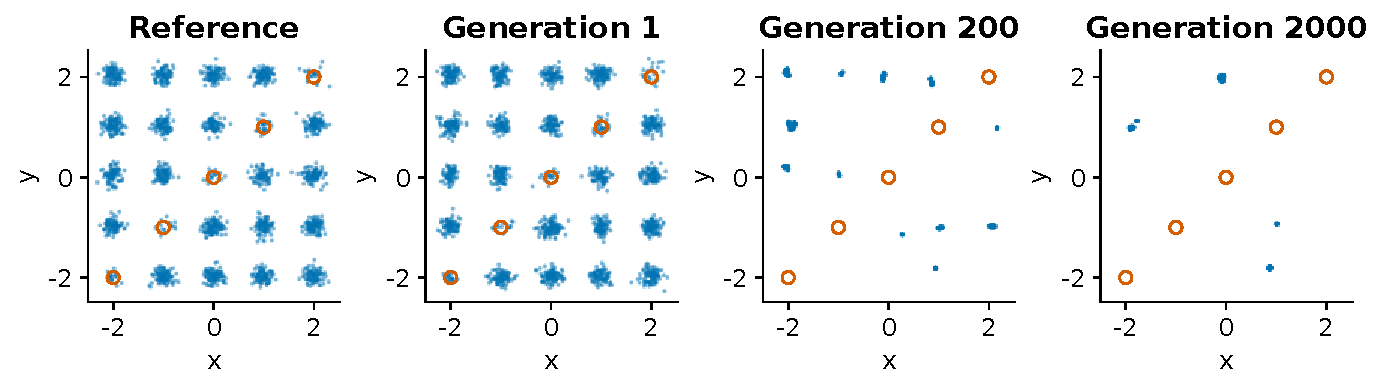
\includegraphics[width=\linewidth]{figures/F01_collapse_snapshots.pdf}
\caption{Distribution evolution in the unbiased fully synthetic loop. Seed 0 is shown at generations 1, 200, and 2,000 alongside the empirical reference. Each panel contains 2,000 points and uses common axes. Orange circles indicate the five rare-component centers.}
\end{figure}

Total covariance trace and mean component covariance trace behave differently during collapse (Figure 2). Component variance drops by more than two orders of magnitude alongside recall, whereas total variance remains much higher because the surviving clusters stay separated across the plane.


\begin{figure}[!htbp]\centering
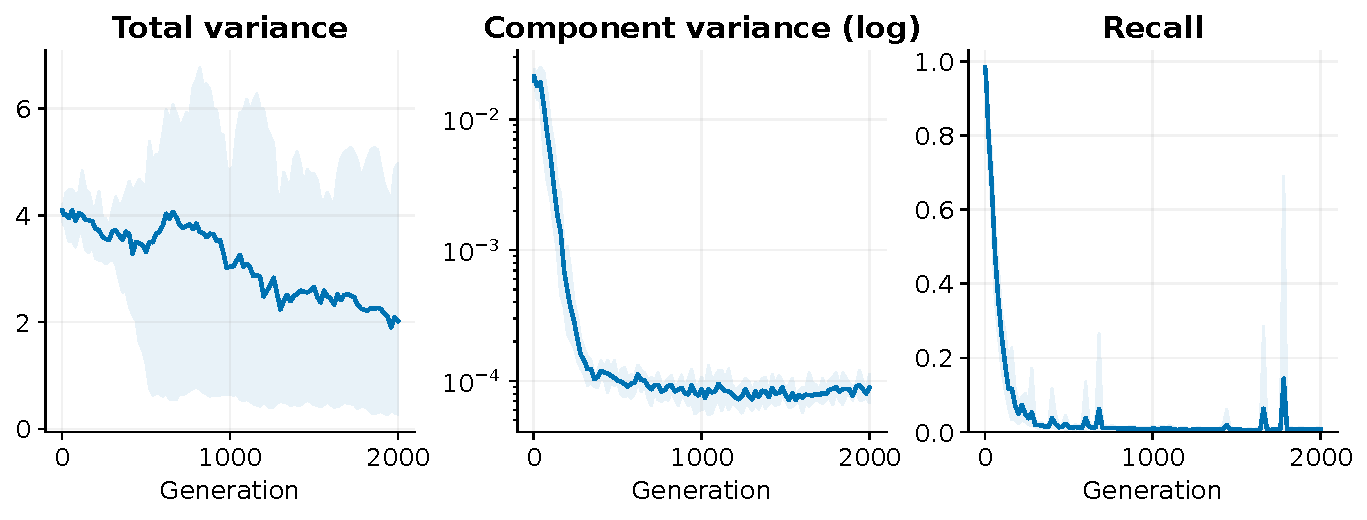
\includegraphics[width=\linewidth]{figures/F02_diversity_metrics.pdf}
\caption{Diversity diagnostics for unbiased fully synthetic training. Total variance includes within-component and between-component variation. The middle panel shows the unweighted mean component covariance trace on a logarithmic axis. Bands show the range across five seeds.}
\end{figure}

\FloatBarrier
\subsection{Persistent real data maintains empirical coverage}

Both regimes that retain real data maintain high recall through generation 2,000 (Figure 3). Fixed-real training ends with mean recall 0.9852 and rare-class recall 0.9892, while the 10\% fresh-real schedule ends at 0.9666 overall and 0.9227 for rare classes. All five seeds in both regimes cover all 25 mode neighborhoods at generation 2,000.


\begin{table}[!htbp]\centering\small

\caption{Generation-2,000 performance averaged over five seeds.}

\begin{tabularx}{\linewidth}{@{}YYYY@{}}\toprule

\textbf{Regime} & \textbf{Recall} & \textbf{Rare-class recall} & \textbf{Fréchet statistic}\\\midrule

Fully synthetic & 0.0076 & 0.0000 & 4.4365\\

Fresh real & 0.9666 & 0.9227 & 0.0201\\

Fixed real & 0.9852 & 0.9892 & 0.0038\\

\bottomrule\end{tabularx}\end{table}

\begin{figure}[!htbp]\centering
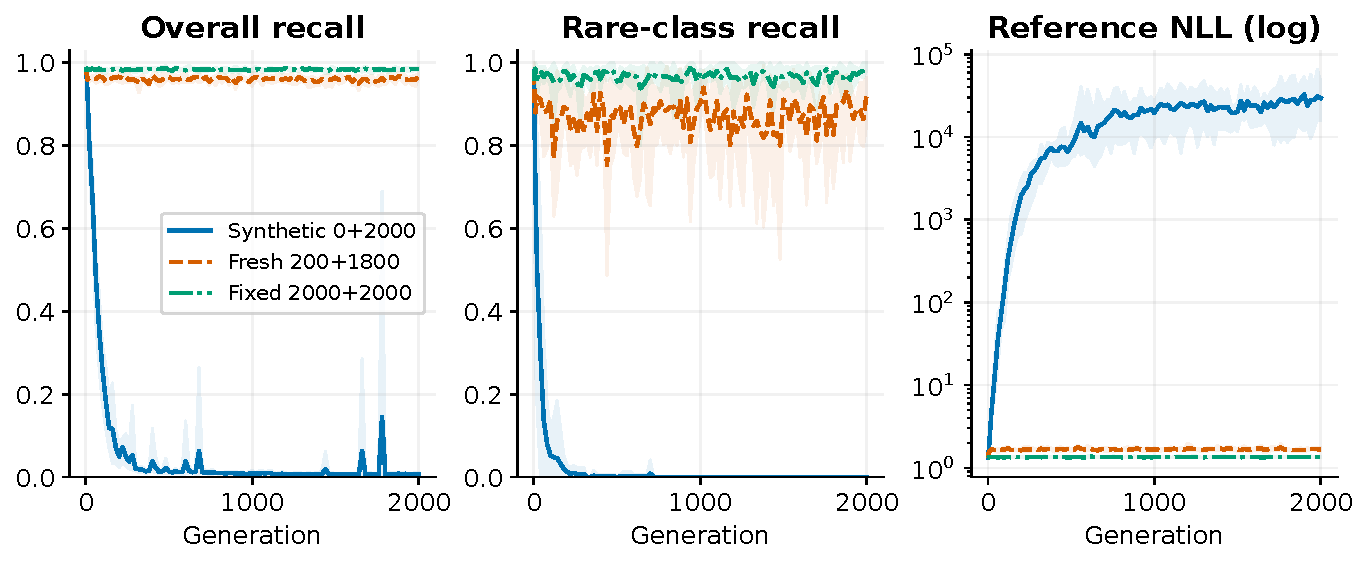
\includegraphics[width=\linewidth]{figures/F03_training_loops.pdf}
\caption{Real-data supply and recursive training. The fully synthetic and fresh-real regimes use 2,000 training observations per generation; the fixed-real regime uses 4,000. The fixed-real training set includes the empirical reference observations.}
\end{figure}

In the fresh-real loop, rare-class recall stays consistently below common-class recall (Figure 4), finishing at 0.9227 versus 0.9695 at generation 2,000. Because rare modes represent only 5\% of the mixture, aggregate recall sits close to the common-class figure. In the fully synthetic loop, rare-class recall also drops to zero earlier than common-class recall.


\begin{figure}[!htbp]\centering
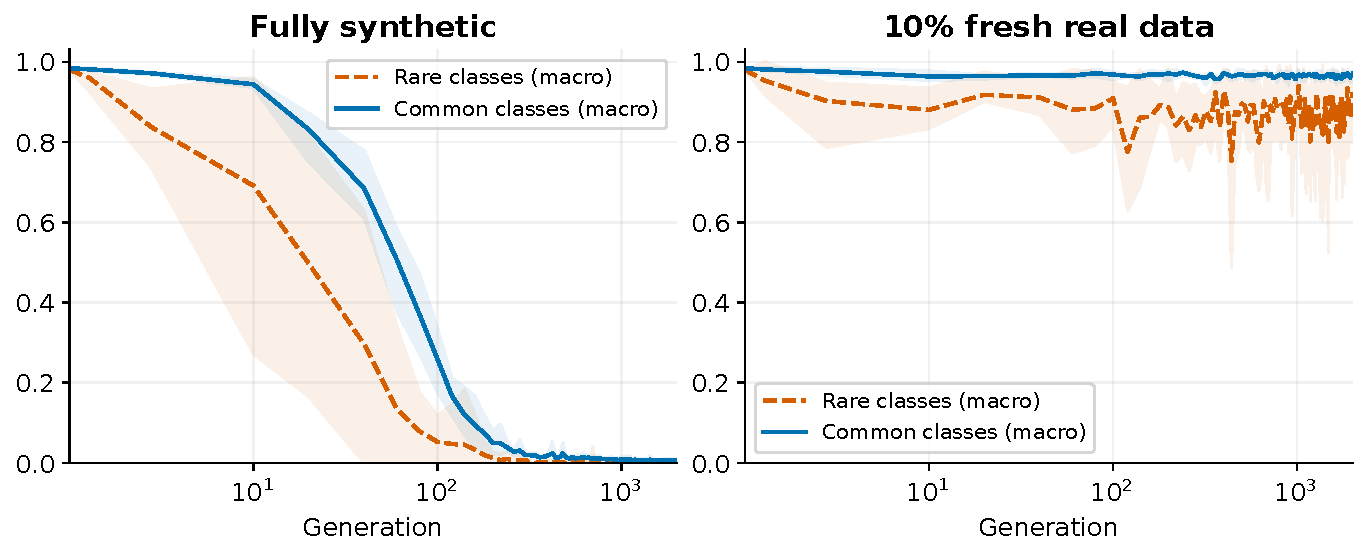
\includegraphics[width=\linewidth]{figures/F04_rare_common.pdf}
\caption{Rare-class and common-class recall under fully synthetic and 10\% fresh-real training. Group summaries use classwise macro-averages. The horizontal axis emphasizes early generations using a symmetric logarithmic scale restricted to positive generations.}
\end{figure}

\FloatBarrier
\subsection{Sampling bias accelerates covariance contraction}

Recall first falls below 0.5 at generations 60--80 under unbiased sampling ($\lambda=1$), at generation 10 for every seed under $\lambda=0.8$, and at generation 5 for every seed under $\lambda=0.5$ (Figure 5). By generation 2,000, both biased conditions reach precision 1.0000 while recall falls to 0.0005 ($\lambda=0.8$) and 0.0000 ($\lambda=0.5$), as generated points contract into tight subsets inside the reference support.


\begin{table}[!htbp]\centering\small

\caption{Generation-2,000 precision and recall under sampling bias.}

\begin{tabularx}{\linewidth}{@{}YYY@{}}\toprule

\textbf{Bias factor} & \textbf{Terminal precision} & \textbf{Terminal recall}\\\midrule

1.0 & 0.9440 & 0.0076\\

0.8 & 1.0000 & 0.0005\\

0.5 & 1.0000 & 0.0000\\

\bottomrule\end{tabularx}\end{table}

\begin{figure}[!htbp]\centering
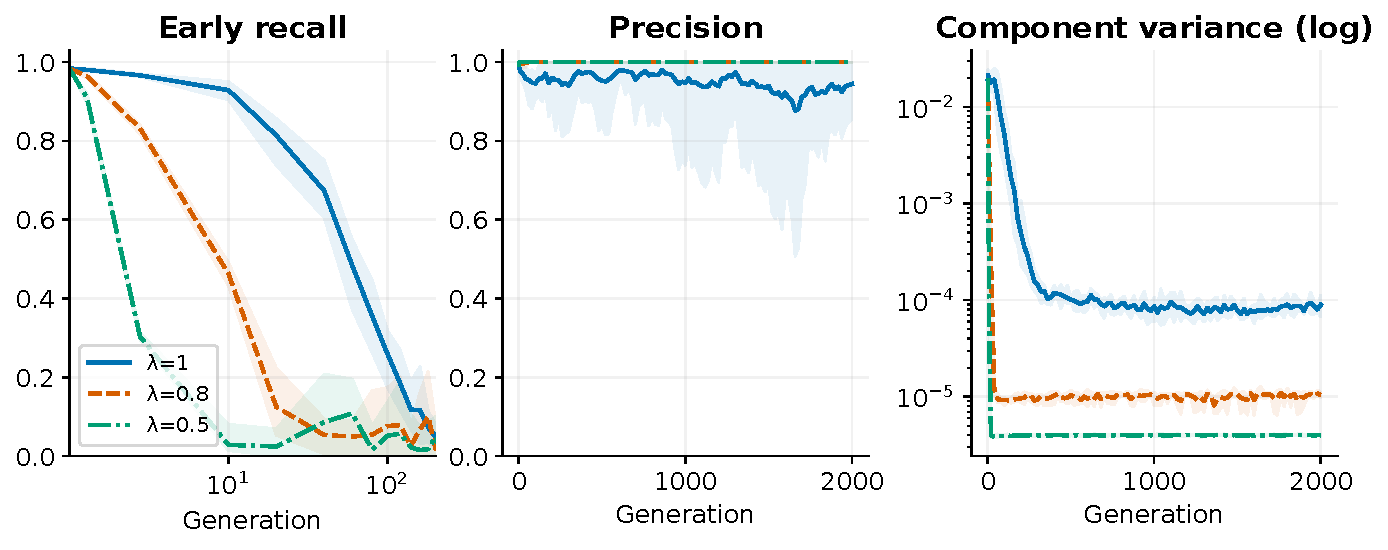
\includegraphics[width=\linewidth]{figures/F05_sampling_bias.pdf}
\caption{Sampling bias and diversity contraction. Bias is applied to training draws through covariance scaling. Recall, precision, and component variance are evaluated using unbiased samples from each fitted model. The recall panel focuses on the first 200 generations.}
\end{figure}

\FloatBarrier
\subsection{Common fresh-data supply reduces initial-model dependence}

Increasing the initial real sample from 500 to 2,000 and 8,000 raises generation-1 recall from 0.9572 to 0.9790 and 0.9819. Once all three runs enter the shared 200-fresh plus 1,800-synthetic schedule, their late-stage metrics converge (Figure 6): across the final 500 generations, mean tail recall lies between 0.9586 and 0.9593, and tail rare-class recall lies between 0.8641 and 0.8774.


\begin{table}[!htbp]\centering\small

\caption{Initial and tail recall under a common fresh-data schedule.}

\begin{tabularx}{\linewidth}{@{}YYYY@{}}\toprule

\textbf{Initial observations} & \textbf{Initial recall} & \textbf{Tail recall} & \textbf{Tail rare-class recall}\\\midrule

500 & 0.9572 & 0.9587 & 0.8641\\

2,000 & 0.9790 & 0.9593 & 0.8712\\

8,000 & 0.9819 & 0.9586 & 0.8774\\

\bottomrule\end{tabularx}\end{table}

\begin{figure}[!htbp]\centering
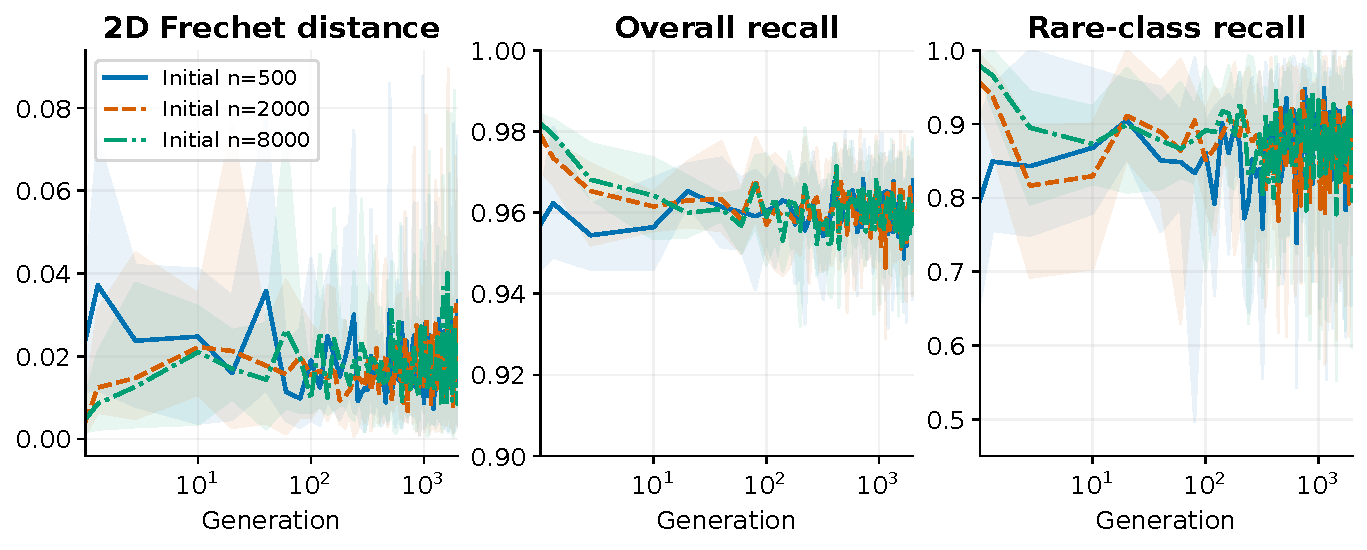
\includegraphics[width=\linewidth]{figures/F06_initial_memory.pdf}
\caption{Initial sample size and recursive performance. Initial GMMs are fitted separately to nested real samples for each seed. All subsequent fits use 200 fresh and 1,800 synthetic observations, with paired random streams across initial sizes.}
\end{figure}

\FloatBarrier
\subsection{Synthetic-data utility depends on sampling bias}

At $n_r=200$, the real-only calibration mean squared sliced Wasserstein distance is 0.03313. Under unbiased sampling ($\lambda=1$), every tested synthetic budget improves on this baseline, though gains flatten out at larger budgets: raising $n_s$ from 1,800 to 3,800 shifts the tail distance only from 0.01869 to 0.01862 (Figure 7).


Under $\lambda=0.8$, synthetic budgets of 200, 800, and 1,800 still reduce the tail distance below 0.03313, but increasing $n_s$ to 3,800 pushes the distance up to 0.05339. For this bias factor and fresh-data budget, synthetic augmentation switches from helpful to harmful between $n_s=1,800$ and $n_s=3,800$.


\begin{table}[!htbp]\centering\small

\caption{Tail squared sliced Wasserstein distance at a fixed fresh budget of 200.}

\begin{tabularx}{\linewidth}{@{}YYY@{}}\toprule

\textbf{Synthetic observations} & \textbf{Tail distance at $\lambda=1$} & \textbf{Tail distance at $\lambda=0.8$}\\\midrule

200 & 0.02456 & 0.02295\\

800 & 0.02006 & 0.02132\\

1,800 & 0.01869 & 0.02212\\

3,800 & 0.01862 & 0.05339\\

\bottomrule\end{tabularx}\end{table}

\begin{figure}[!htbp]\centering
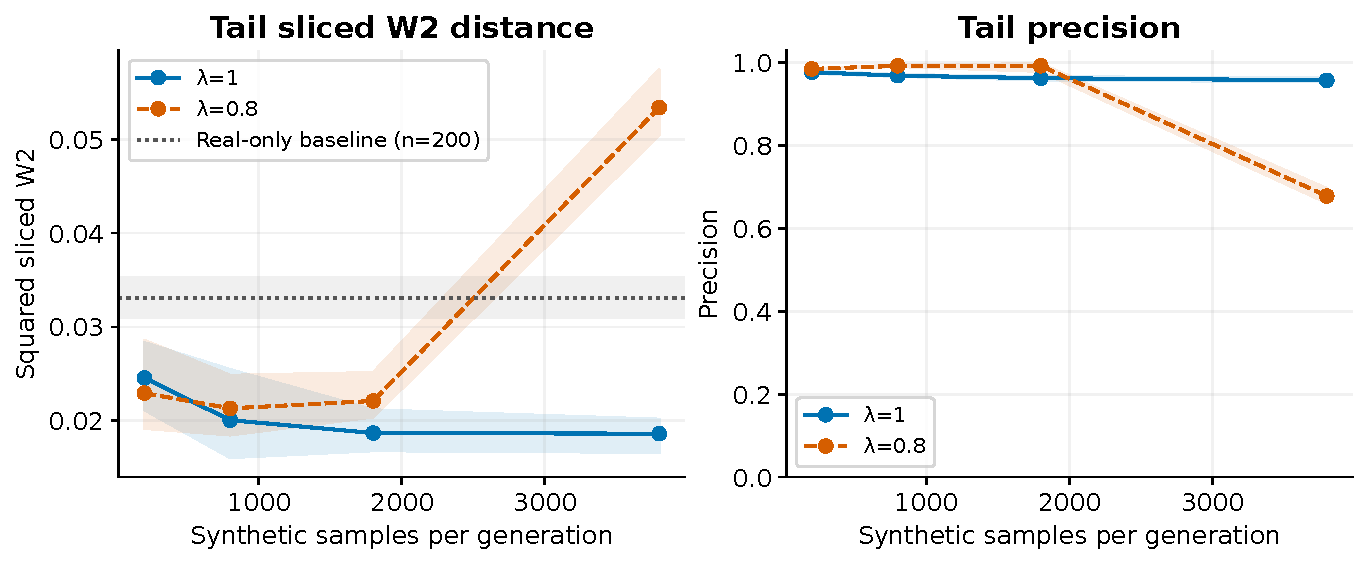
\includegraphics[width=\linewidth]{figures/F07_synthetic_benefit.pdf}
\caption{Synthetic-data utility at a fixed fresh budget of 200 observations per generation. Distances and precision are averaged over each seed's last 500 generations and then across seeds. Colored bands show seed ranges; the gray band shows the real-only calibration mean plus or minus one standard error.}
\end{figure}

Among the tested conditions, $\lambda=0.8$ with $n_s=1,800$ meets the tail stability criterion across all five seeds. Its tail distance of 0.02212 matches a real-only training size of approximately 348 observations (Figure 8), giving an effective-to-fresh sample ratio of 1.74.


\begin{figure}[!htbp]\centering
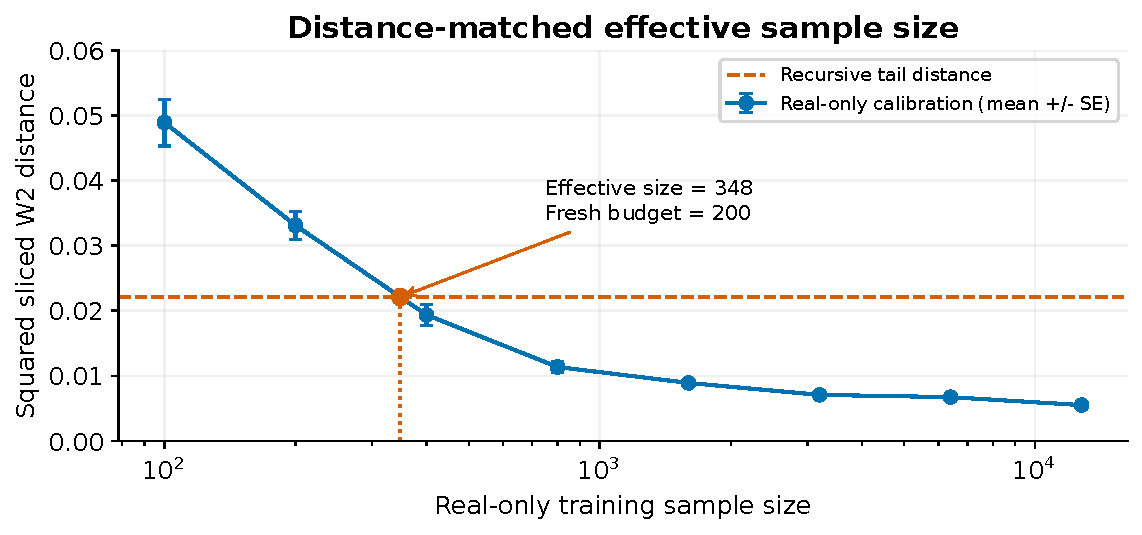
\includegraphics[width=\linewidth]{figures/F08_effective_sample_size.pdf}
\caption{Distance matching for effective sample size. The real-only calibration uses 50 fits per sample size. The recursive tail distance for 200 fresh and 1,800 synthetic observations at bias factor 0.8 intersects the calibration curve at approximately 348 real observations.}
\end{figure}

\FloatBarrier
\section{Discussion}

The two real-data regimes maintain coverage in different ways. Fixed-real training reuses the original 2,000 observations at every step alongside 2,000 synthetic points, keeping the empirical reference directly in the training set with a larger total sample size (4,000). Fresh-real training draws 200 new independent observations per generation for a total size of 2,000. Under this 10\% fresh schedule, each rare component receives 2 fresh observations per generation in expectation, compared with 9.5 for each common component, which accounts for the persistent gap between rare-class and common-class recall.


The rapid collapse under biased sampling follows from repeated covariance scaling. For an isolated component that retains non-negligible weight, the covariance update is approximately $\Sigma_{t+1}\approx\lambda\Sigma_t+\varepsilon I_2$, which approaches a trace of $2\varepsilon/(1-\lambda)$. With $\varepsilon=10^{-6}$, this gives $10^{-5}$ at $\lambda=0.8$ and $4\times10^{-6}$ at $\lambda=0.5$, matching the late-stage component traces in Figure 5. Because samples shrink toward the interiors of existing modes, generated points remain inside the reference neighborhood balls (keeping precision near 1) while covering fewer reference points (driving recall toward 0).


Total covariance trace does not separate within-component shrinkage from between-component spread because


\begin{equation}
\operatorname{tr}\operatorname{Cov}(X)=\sum_k w_k\operatorname{tr}\Sigma_k+\sum_k w_k\|\mu_k-\overline\mu\|^2.
\end{equation}

Even after most modes disappear and surviving components contract, the second term stays large whenever the remaining clusters lie far apart. Tracking recall and mean component covariance trace directly shows within-mode collapse that total variance misses.


In the synthetic-budget experiment, unbiased synthetic samples carry information from prior real draws and reduce estimation error relative to fitting on 200 fresh points alone, with diminishing marginal improvement as $n_s$ grows. Under $\lambda=0.8$, moderate synthetic counts still reduce variance enough to beat the real-only baseline, but at $n_s=3,800$ the bias from covariance shrinkage outweighs that gain and worsens the fitted distribution.


\clearpage

\FloatBarrier
\section{Conclusion}

In this 25-component imbalanced Gaussian mixture, fully synthetic recursive training drives recall to 0.0076 and eliminates all rare-class recall within 2,000 generations. Keeping real data in the loop, either by reusing the initial sample or by supplying 10\% fresh observations per generation, preserves all 25 modes and keeps overall recall above 0.96, although rare components still lag common components under limited fresh data. Covariance-biased sampling moves recall collapse from generations 60--80 to generations 5--10 while keeping precision at 1.0000. Under a shared fresh-data schedule, initial sample sizes from 500 to 8,000 converge to nearly the same late-stage recall. When fresh data is fixed at 200 points per generation, unbiased synthetic augmentation improves distributional accuracy with diminishing returns, whereas biased augmentation ($\lambda=0.8$) helps up to 1,800 synthetic points before degrading accuracy at 3,800.


\FloatBarrier\begin{thebibliography}{9}

\bibitem{r1}S. Alemohammad, J. Casco-Rodriguez, L. Luzi, A. I. Humayun, H. Babaei, D. LeJeune, A. Siahkoohi, and R. G. Baraniuk, Self-Consuming Generative Models Go MAD, arXiv:2307.01850 (2023).

\bibitem{r2}M. Heusel, H. Ramsauer, T. Unterthiner, B. Nessler, and S. Hochreiter, GANs Trained by a Two Time-Scale Update Rule Converge to a Local Nash Equilibrium, in \emph{Advances in Neural Information Processing Systems} \textbf{30} (2017), pp. 6626--6637.

\bibitem{r3}T. Kynkäänniemi, T. Karras, S. Laine, J. Lehtinen, and T. Aila, Improved Precision and Recall Metric for Assessing Generative Models, in \emph{Advances in Neural Information Processing Systems} \textbf{32} (2019), pp. 3929--3938.

\end{thebibliography}

\end{document}
